%!TEX root = ../doc.tex
\chapter{Implementation}
\label{sec:Implementation}
This chapter describes the implementation and the connections of the individual components of the augmented reality system. There are two main tasks, the system needs to perform: A three dimensional estimation of the surrounding and the precise measurement of motion of the camera head.
\section{Video inputs}
The system utilizes two cameras, a Raspberry Pi Camera v2 and a PiEye ToF camera that doubles as an infrared camera. The Sony IMX 219 based Raspberry Pi Camera v2 features a color image with an 8 megapixel resolution for single images, 1080p with 30 frames per second, 720p with 60 frames per second or 480p with 90 frames per second.\cite{raspiCamSpec} The Raspberry Pi Camera v2 is a Mipi CSI2 attached camera module whichs cable length got extended by an FPDLink serializer and deserializer.\\
The PiEye ToF camera is based on the Infineon REAL3 IRS1125A sensor which has a resolution of 352 x 288 pixels\cite{piEyeShop}. The ToF Camera is paired with infrared LED flashes to measure the time of flight of the light emitted and has an intended measurement range from 10 centimeters up to five meters. The entire ToF software stack runs on a Raspberry Pi that sends its video data via Ethernet to the augmented reality system.\\


\subsection{ToF Camera calibration}
\label{sec:ToFCalibration}
On the ToF Camera, two parts need to be calibrated: The optics, as described in section \ref{sec:FundCamCalibration}, and the distance measurement. The ToF camera has a barrel type distortion that is corrected by the camera calibration algorithm implemented in OpenCV\cite{openCVCamCalib} and shown in image \ref{fig.camCalib}. As the process of lens correction cuts off parts of the image, the image size gets lowered to 265 x 205 pixels.\\
For the distance measurement, first the radial distances need to be flattened as described in section \ref{sec:RadialCorrection}. As the angle $\alpha$ is not known for each pixel, a reference measurement provides the necessary information. To reduce noise, 19 images of the same flat wall has been taken, smoothed by a gaussian and averaged onto one reference image $I_{Ref}$. The wireframe image in figure \ref{im:ToFRaw} shows the curvature of the reference image. The rounding at the edges is an arfifact of the gaussian smoothing.\\
\begin{figure}[H]
    \centering
    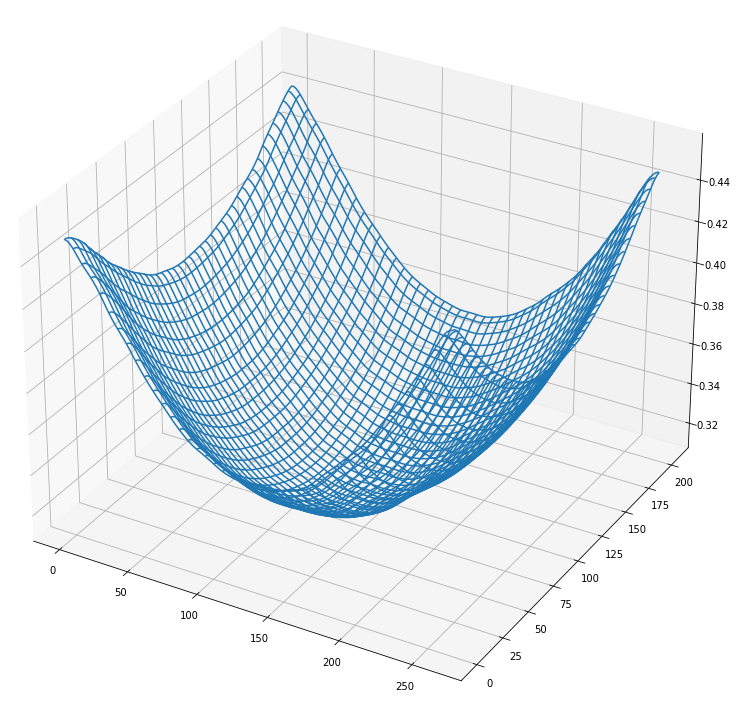
\includegraphics[width=0.4\textwidth]{images/raw_tof_radial.png}
    \caption{Wireframe rendering of the reference image $I_{Ref}$ provided by the ToF camera}
    \label{im:ToFRaw}
\end{figure}
Dividing the minimum value of this reference image $I_{Ref}$ with every pixel value generates a map of $\cos \alpha$ named $I_{cos}$.
\begin{equation*}
    I_{cos} = \frac{\min (I_{Ref}) }{I_{Ref}} 
\end{equation*}
Pixel by pixel multiplication of any other image $I_{Any}$ with $I_{cos}$ will correct the influence of the radial measurement as shown in image \ref{im:ToFCorrected}. 
\begin{equation*}
    I_{Corr} = I_{cos}\cdot I_{Any}
\end{equation*}
\begin{figure}[H]
    \centering
    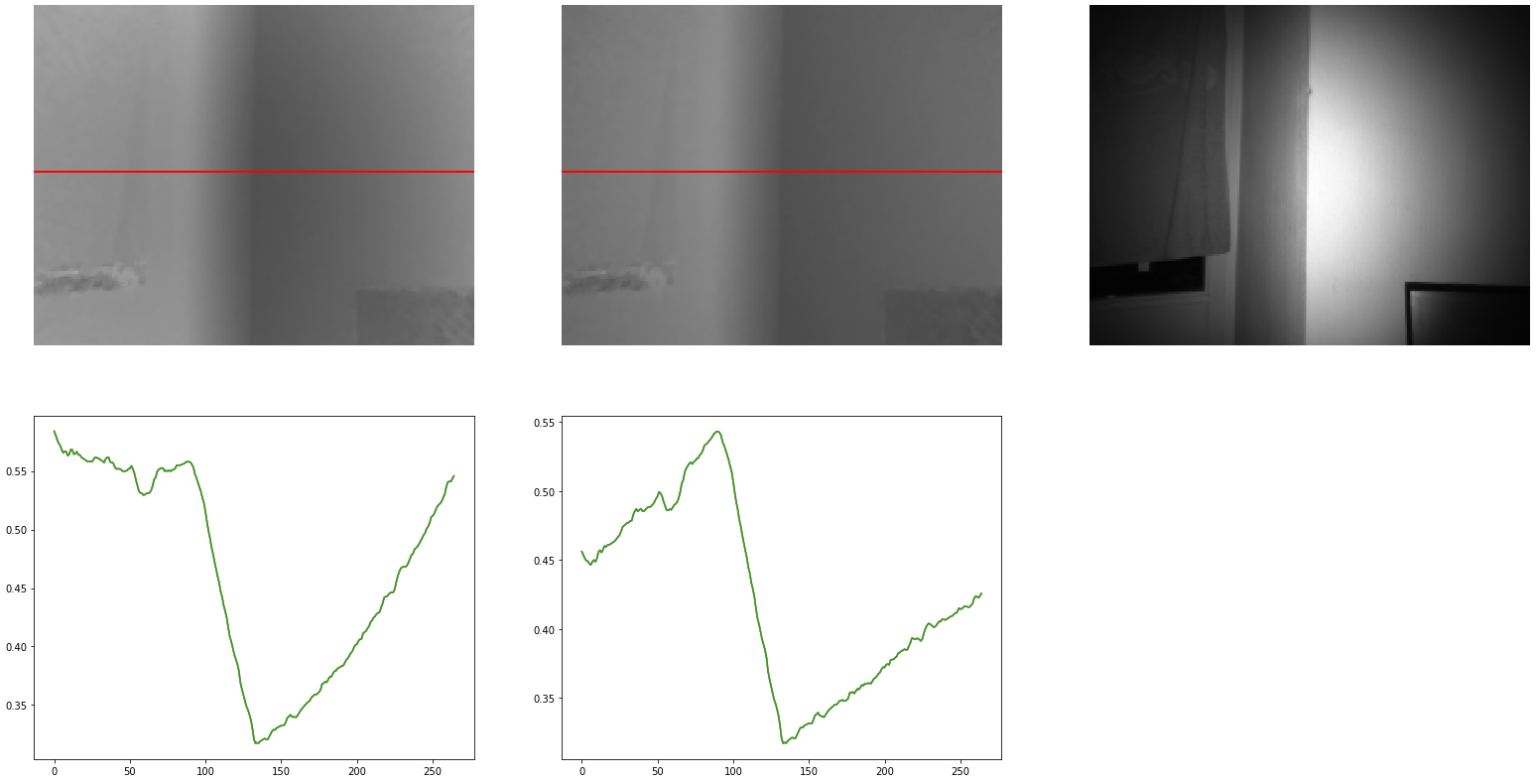
\includegraphics[width=1.0\textwidth]{images/flattened_tof_example.png}
    \caption{Left, the uncorrected ToF image $I_{Any}$, in the middle the corrected image $I_{Corr}$ and on the right, the infrared grayscale image of the scene. To make the effect more apparent, the brightness accross the red lines have been plotted.}
    \label{im:ToFCorrected}
\end{figure}


TODO: Distance measurement calibration!
\subsection{Raspberry Pi Camera calibration}
\label{sec:RBPiCalibration}
TODO: Cam calibration
\section{Gyroscope and Accelerometer Calibration}
\label{sec:GyroCal}
The used inertial movement unit (IMU) is a Bosch BMI160, that is sold soldered on a PCB by DFRobot.\\
As the gyroscope and accelerometer output incremental movement, the values need to be integrated over time. Accurate data is crucial for finding the direction of gravity or detecting movement - especially because of positional information being the result of derivating the acceleration twice.\\
The range of the acclerometer is variable and has been set to ±8 G, it has an output resolution of 16 bit and an output data rate of 200 Hz.
The accelerometer has been calibrated in 24 orientations to even out angle errors inside the IMU, on the PCB and of the calibration table, as shown im image \ref{im:IMU_cal}. For each orientation, 100 raw measurements have been averaged to even out noise. 
\begin{figure}[H]
    \centering
    
\includegraphics[width=1.0\textwidth]{images/todo.png}
    \caption{The 24 orientations used for calibration - four directions for each of the six sides.}
    \label{im:IMU_cal}
\end{figure}
The largest error has been 38 mG, that lies within the sensor's specification of ±40 mG\cite{BMI160}. In addition, the gain for the accelerometer has been corrected based on gravity. A maximum error of 1.8\% has been measured and corrected, which also lies in the sensor's specification of ±0.5\% full scale\cite{BMI160}.\\
For the gyroscope, the range is set to ±2000 degrees per second with an output data rate of 200 Hz. The gyroscope has been calibrated only for zero offset, whose maximum error was 0.2 degrees per second which lies well in the specified ±3 degrees per second\cite{BMI160}. A gain correction was not made, because of not having the required equipment to do so.\\
\section{Position estimation}
\label{sec:PositionEstimate}
The position estimation of the camera head is crucial for the augmented reality platform. 
\subsection{Gyroscope and Accelerometer}
\label{sec:GyroPosition}
TODO: Position estimate fast
\subsection{SIFT features movement detection}
\label{sec:SIFTPosition}
TODO: Position estimate slow
\subsection{Sensor Fusion with Kalman Filter}
\label{sec:SIFTPosition}
TODO: Position estimate slow
\section{Video display}
\label{sec:VideoDisplay}
TODO: Vulkan Output